\newpage
\section{Patinete eléctrico}
\label{anexo_patienete eléctrico}

Los patinetes eléctricos son una alternativa como medio de transporte que ha ido ganando popularidad entre los ciudadanos dado su bajo coste frente a otros medios más convencionales y la libertad de movilidad que ofrece.

Actualmente, no existe una normativa que abarque a todas las comunidades autónomas de España, sin embargo, existe una normativa básica proporcionada por la \gls{dgt} \cite{dgtpatinete,recomendacionespatinete,instrucciondgt}, donde se recogen normas establecidas en algunas de las ciudades principales de España, como Barcelona, Madrid o Sevilla.

Basándonos en la normativa generalizada de la \gls{dgt} se deben cumplir las siguientes normas para poder circular con los patinetes eléctricos:
\begin{itemize}
    \item El conductor debe tener como mínimo 16 años de edad.
    \item El patinete debe estar provisto de luces frontales y traseras, tal y como lo llevan las motos, y deberán emplearse siguiendo las normas de circulación.
    \item No es obligatorio el uso de casco o chaleco reflectante, a menos que se utilice en carreteras, donde si será obligatorio el uso de chaleco reflectante.
    \item Dado el tipo de vehículo no es obligatorio poseer seguro, pero se recomienda tener uno en caso de accidentes \cite{noticiasegurospatinete,noticiasegurospatinete2}.
    \item Solo pueden circular por los carriles 30 designados, carriles bicis, o en su defecto por acera en caso de no existir alguna de las dos alternativas anteriores, siempre y cuando se reduzca la velocidad y se le dé preferencia a los peatones.
    \item La velocidad máxima por carretera es de 25 \glssymbol{km}/\glssymbol{hora}
    \item Solo pueden aparcarse en las zonas especiales \cite{aparcamientopatinete,aparcamientopatinetemapa} designadas para patinetes eléctricos (véase imagen/mapa o tabla), o en su defecto, zonas donde no molesten o se empleen mobiliario público.
\end{itemize}

Por otro lado, hay que tener en consideración las multas \cite{normativapatinete} que pueden recibir los conductores. Las cantidades pueden diferir, pero las posibles multas son:
\begin{itemize}
    \item Circular por aceras o zonas de peatones donde existe carril, bici o carretera - 200 \glssymbol{euro}
    \item Aparcar fuera de zona de estacionamiento: 200 \glssymbol{euro}
    \item Uso de teléfono o cascos de audio mientras se conduce: 200 \glssymbol{euro}
    \item Llevar dos pasajeros: 90 \glssymbol{euro}
    \item No llevar casco o chaleco en zonas obligatorias: 90 \glssymbol{euro}
    \item Exceder velocidad máxima: 200 \glssymbol{euro}
    \item Consumo de drogas, alcohol o conducción temerosa: 500-1000 \glssymbol{euro}
\end{itemize}

El conductor no está obligado a poseer carné de conducción de patinetes, pero debe tener bajo su poder, bien sea en documento físico o documento electrónico, el certificado \gls{ce} y ficha técnica del vehículo \cite{cetallerdelpatinete}, proporcionado por cada empresa vendedora de patinetes. En las \autoref{fig:CE patinete 1} y \autoref{fig:CE patinete 2} \cite{ceejemplo} se recogen como debe de ser un certificado \gls{ce}.

\begin{figure}[H]
    \centering
    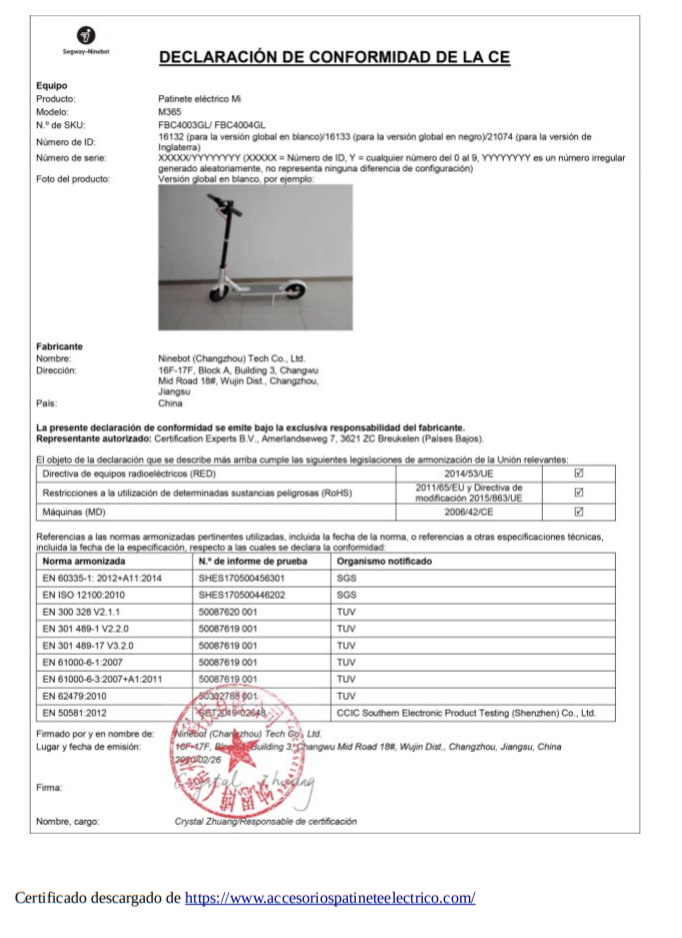
\includegraphics[scale=0.8]{archivos/CE patinete 1.png}
    \caption{\gls{ce} Patinete - Parte 1.}
    \label{fig:CE patinete 1}
\end{figure}

\begin{figure}[H]
    \centering
    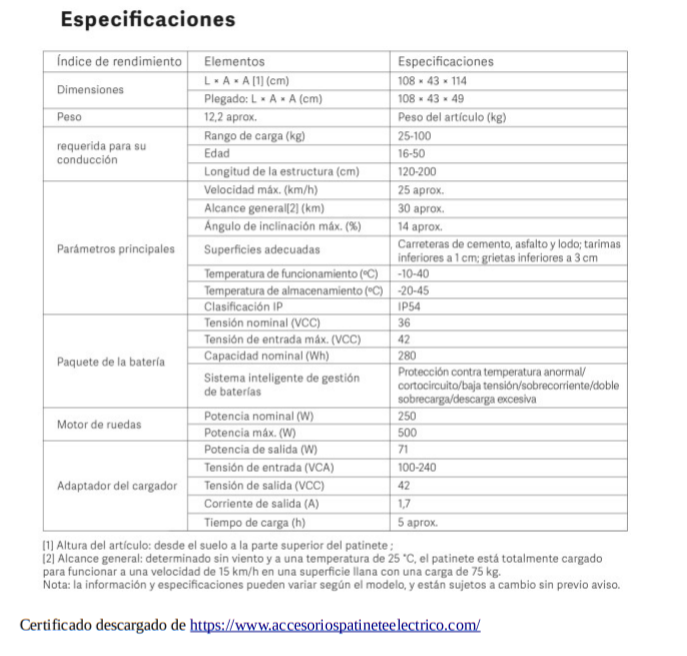
\includegraphics[scale=0.8]{archivos/CE patinete 2.png}
    \caption{\gls{ce} Patinete - Parte 2.}
    \label{fig:CE patinete 2}
\end{figure}

En la \autoref{tabla: modelo_patinete_electrico} se recogen algunos modelos de patinetes eléctricos existentes en el mercado actualmente, junto con algunas de sus características más destacables para el estudio.

\begin{table}[h]
\centering
\resizebox{1\textwidth}{!}{%
\begin{tabular}{|l|c|c|c|c|c|c|c|c|c|c|}
\hline
\multicolumn{1}{|c|}{\textbf{Modelo}} & \textbf{\begin{tabular}[c]{@{}c@{}}Autonomía\\ (\glssymbol{km})\end{tabular}} & \textbf{\begin{tabular}[c]{@{}c@{}}Vel. máx.\\ (\glssymbol{km}/\glssymbol{hora})\end{tabular}} & \textbf{\begin{tabular}[c]{@{}c@{}}Carga máx.\\ (\glssymbol{kg})\end{tabular}} & \textbf{\begin{tabular}[c]{@{}c@{}}Escalada máx\\ (\%)\end{tabular}} & \textbf{\begin{tabular}[c]{@{}c@{}}Absorción\\ choque\end{tabular}} & \textbf{\begin{tabular}[c]{@{}c@{}}Resistencia\\ al agua\end{tabular}} & \textbf{\begin{tabular}[c]{@{}c@{}}Potencia\\ (\glssymbol{vatios})\end{tabular}} & \textbf{\begin{tabular}[c]{@{}c@{}}Tiempo\\ carga (\glssymbol{hora})\end{tabular}} & \textbf{\begin{tabular}[c]{@{}c@{}}Capacidad\\ (\glssymbol{vatiohora})\end{tabular}} & \textbf{\begin{tabular}[c]{@{}c@{}}Precio\\ (\glssymbol{euro})\end{tabular}} \\ \hline
\textbf{\begin{tabular}[c]{@{}l@{}}Xiaomi Mi Electric \\ Scooter 3 Negro\end{tabular}} & 30 & 25 & 100 & 16 & Si & ?? & 600 & 5,5 & 275 & 427,47  \\ \hline
\textbf{\begin{tabular}[c]{@{}l@{}}Segway Ninebot KickScooter \\ F30E Patinete Eléctrico 10"\end{tabular}} & 30 & 25 & 120 & 15 & No & Si & 300 & 6,5 & 367 & 435,00  \\ \hline
\textbf{\begin{tabular}[c]{@{}l@{}}Segway Ninebot KickScooter \\ F40E Patinete Eléctrico 10"\end{tabular}} & 40 & 25 & 120 & 20 & No & Si & 350 & 6,5 & 367 & 504,99  \\ \hline
\textbf{\begin{tabular}[c]{@{}l@{}}Xiaomi Mi Electric Scooter \\ 1S Patinete Eléctrico Negro\end{tabular}} & 30 & 25 & 100 & 14 & Si & Si & 500 & 5,5 & 275 & 380,48  \\ \hline
\textbf{\begin{tabular}[c]{@{}l@{}}Infiniton CITYJam Pro \\ Patinete Eléctrico Negro\end{tabular}} & 40 & 25 & 100 & 15 & Si & Si & 350 & 6,5 & 350 & 376,62  \\ \hline
\end{tabular}%
}
\caption{Modelos de patinetes eléctricos.}
\label{tabla: modelo_patinete_electrico}

\end{table}

\newpage
% \addcontentsline{toc}{section}{Referencias}
% \section*{Referencias}
% \label{referencias_nucleo}
% \makeatletter
% \def\@bibitem#1{\item\if@filesw \immediate\write\@auxout
%   {\string\bibcite{#1}{A\the\value{\@listctr}}}\fi\ignorespaces}
% \def\@biblabel#1{[A{#1}]}
% \makeatother
% \printbibheading[title={Referencias},heading=bibintoc]
\nocite{*}
\newrefcontext[labelprefix=\thesection.]
\printbibheading[title={Referencias},heading=subbibintoc]
\printbibliography[heading=none,resetnumbers=true,keyword=patineteelec]
\newpage
